\documentclass{article}
\usepackage[pdftex]{graphicx}
\usepackage{parskip}
\begin{document}

\huge{Instituto Politecnico Nacional}
\bigskip
\bigskip
\bigskip
\\
\LARGE{Escuela Superior De C\`omputo}
\bigskip
\bigskip
\bigskip
\\
\LARGE{Materia: Ingenieria del Software}
\bigskip
\bigskip
\bigskip
\\
\LARGE{Profesora: Reyna Melara}
\bigskip
\bigskip
\bigskip
\\
\Large{Practica 3}
\bigskip
\bigskip
\bigskip
\\
\Large{Alumnos: Mart\`inez Rend\`on Diego Alberto}
\bigskip
\\
\Large{ Jim\`enez Flores Javier}
\bigskip
\bigskip
\\
\Large{Grupo: 3CV2}
\bigskip
\\
\newpage
\huge{Indice}
\bigskip
\bigskip
\\
\bigskip
\bigskip
\\
\LARGE{Desarrollo			.	.	.	.	.	.	.	.	3}
\bigskip
\bigskip
\\
\LARGE{Conclusi\`on			.	.	.	.	.	.	.	.	4}
\bigskip
\\
\newpage
\huge{Desarrollo}
\bigskip
\\
\normalsize{Deacuerdo con las especificaci\`ones de la practica, Se prosiguio a desarrollar un programa para la validaci\`on de cadenas de texto en formato de direcci\`on URL.}
\\
\normalsize{Se nos pidio responder a los siguientes cuestionamientos:}
\bigskip
\\
\normalsize{Aproximadamente �cu\`antas pruebas realiz\`o de su programa\?.} 
\bigskip
\\
\normalsize{Aproximadamente 12 pruebas se realizaron.}
\bigskip
\\
\normalsize{�En cu\`anto tiempo resolvi\`o el problema\?} 
\bigskip
\\
\normalsize{Debidamente dedicados 30 minutos}
\bigskip
\\
\normalsize{�Cu�ntos cambios se requirieron de la primer propuesta del c\`odigo\?} 
\bigskip
\\
\normalsize{Dos cambios}
\bigskip
\\
\normalsize{�Los datos de prueba que se proporcionaron fueron aprobados\?} 
\bigskip
\\
\normalsize{Afirmativo fue aprobado}
\bigskip
\\
\normalsize{�Qu\`e convenciones de codificaci\`on eligi\`o con su par de programaci\`on\?} 
\bigskip
\\
\normalsize{Ninguna}
\bigskip
\\
\normalsize{�A qu\`e se refiere el t\`ermino TestDriven development\?} 
\bigskip
\\
\normalsize{Desarrollo basado en prueba y error de la aplicaci\`on}
\bigskip
\\
\normalsize{�Qu\`e beneficios tiene la programaci\`on en pares\?} 
\bigskip
\\
\normalsize{Correcci\`on de errores y diseno e implementaci\`on al mismo tiempo}
\bigskip
\\
\normalsize{�Qu� desventajas considera que existen de la programaci\`on en pares\?} 
\bigskip
\\
\normalsize{Falta de interacci\`on con los otros miembros del equipo, aislamiento y monotomia}
\bigskip
\\
\normalsize{�Qu\`e porcentaje del c\`odigo escribi\`o cada integrante\?} 
\bigskip
\\
\normalsize{0 \% Mart\`inez Rend\`on Diego Alberto, 100 \% Jim\`enez Flores Javier }
\bigskip
\\
\normalsize{El desarrollo posterior del codigo se puede apreciar en la siguente imagen, se requiere de programacion de jsp para hacer funcionar el codigo propiamente y introducir el codigo en el metodo doPost en el servlet:}

\begin{figure} [h]
\begin{center}
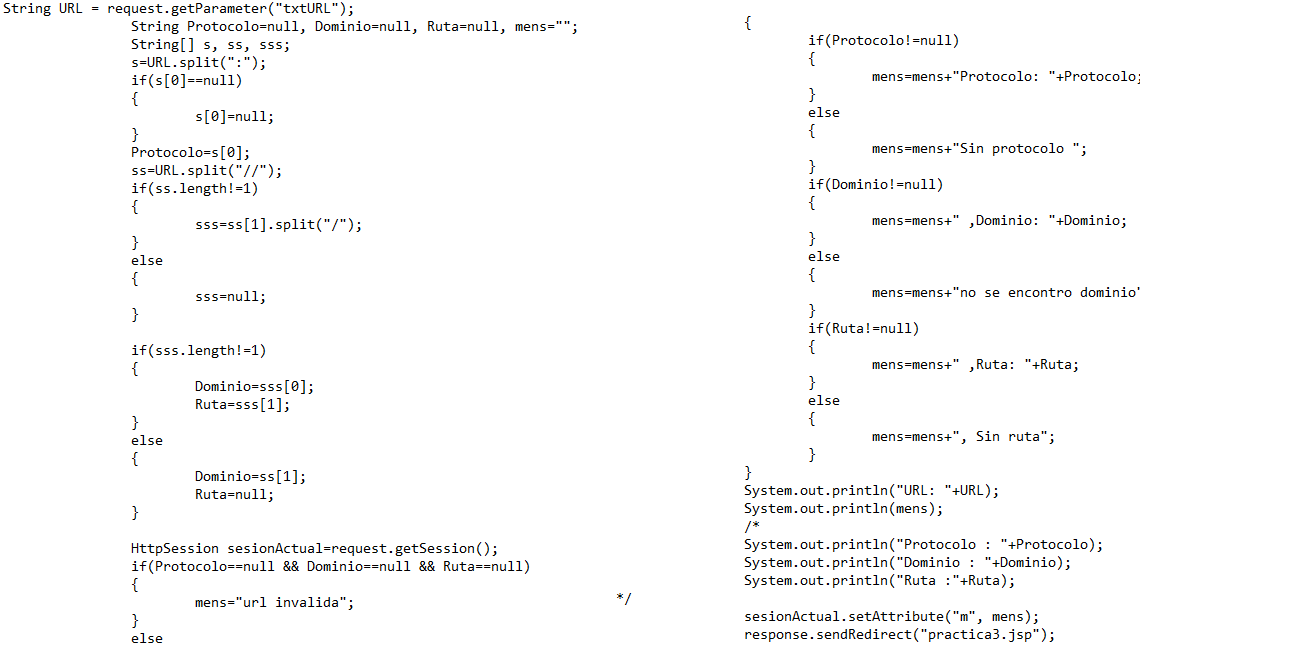
\includegraphics[width=4in,height=4in]{Codigo.png}
\end{center}
\end{figure}


\newpage
\huge{Conclusi\`on}
\bigskip
\\
\normalsize{Diego: El desarrollo tiene sus ventajas y desventajas, es eficiente para resolver un problema express pero no lo es para aplicaciones que requieren de un seguimiento a largo plazo}
\\
\normalsize{Javier: No sirve la metodologia si se siguen demaciodos protocolos de estandarizacion y documentacion en ese caso seria denominado Extreme Programing y no TestDriven}

\\
\end{document}